\documentclass[14pt]{extarticle}
\usepackage{fontspec}
\usepackage{polyglossia}
\usepackage{amsmath}
\usepackage{amssymb}
\usepackage{xcolor}
\usepackage{fancyhdr}
\usepackage{graphicx}
\usepackage{listings}
\usepackage[most]{tcolorbox}
% \usepackage{setspace}
\usepackage{pifont}
\usepackage{enumitem}
\usepackage{titlesec}
\usepackage[bottom]{footmisc}
\usepackage{titling}
\usepackage{minted}
\usepackage{etoolbox}
\usepackage{array}
\usepackage{extsizes}
\usepackage{float}
\usepackage{booktabs}
\usepackage{hyperref}
\usepackage[onehalfspacing]{setspace}
\usepackage[a4paper, top=2.7cm, bottom=2.7cm, left=2.5cm, right=2.5cm, headheight=1.5cm, headsep=0.5cm]{geometry}
\usepackage{tikz}

\usetikzlibrary{automata, positioning, arrows.meta, arrows}

\newfontfamily\emoji{Segoe UI Emoji}

\pagestyle{fancy}

\setmainlanguage[numerals=western]{arabic}
\setotherlanguage{english}
% \newfontfamily\arabicfont[Script=Arabic]{Amiri}
\newfontfamily\arabicfont[Script=Arabic]{Calibri}
\newfontfamily\arabicfonttt[Script=Arabic]{Courier New}

\lstset{
  language=[Sharp]C,
  numbers=left,
  stepnumber=1,
  numbersep=8pt,
  frame=single,
  basicstyle=\ttfamily\small,
  keywordstyle=\color{blue},
  stringstyle=\color{red},
  commentstyle=\color{green!50!black}
}

\newif\ifdetailed
\ifdefined\setdetailed
  \setdetailed
\fi

\newif\ifwithsols
\ifdefined\setwithsols
  \setwithsols
\fi

% unified tcolorboxes for articles
\tcbset{colback=white, colframe=black, fonttitle=\bfseries, boxrule=0.8pt}
\newtcolorbox{boxDef}[1][]{colback=blue!5!white,colframe=blue!75!black,
  title={{\emoji📘} تعريف\ifx\\#1\\\else ~#1\fi :}}
\newtcolorbox{boxExercise}[1][]{colback=cyan!5!white,colframe=cyan!70!black,
  title={{\emoji🧩} تمرين\ifx\\#1\\\else ~#1\fi :}}
\newtcolorbox{boxExample}[1][]{colback=yellow!5!white,colframe=orange!90!black,
  title={{\emoji📝} مثال\ifx\\#1\\\else ~#1\fi :}}
\newtcolorbox{boxNote}[1][]{colback=gray!10!white,colframe=black,
  title={{\emoji✨} ملاحظة\ifx\\#1\\\else ~#1\fi :}}
\newtcolorbox{boxAttention}[1][]{colback=magenta!10!white,colframe=magenta!80!black,
  title={{\emoji🔔} تنبيه\ifx\\#1\\\else ~#1\fi :}}
\newtcolorbox{boxWarning}[1][]{colback=red!5!white,colframe=red!75!black,
  title={{\emoji⚡} ملاحظة هامة\ifx\\#1\\\else ~#1\fi :}}
\newtcolorbox{boxSolution}[1][]{colback=green!5!white,colframe=green!60!black,
  title={{\emoji✅} حل\ifx\\#1\\\else ~#1\fi :}}
\newtcolorbox{boxSymbol}[1][]{colback=purple!5!white,colframe=purple!70!black,
  title={{\emoji🔣} رمز\ifx\\#1\\\else ~#1\fi :}}
\newtcolorbox{boxHint}[1][]{colback=teal!5!white,colframe=teal!60!black,
  title={{\emoji💡} تلميح\ifx\\#1\\\else ~#1\fi :}}


\tcbset{simplecode/.style={ colback=gray!5, colframe=black!50, boxrule=0.4pt, arc=2pt, left=4pt,right=4pt,top=4pt,bottom=4pt}}
\newenvironment{boxCode}{\begin{tcolorbox}[simplecode]}{\end{tcolorbox}}

\newcolumntype{C}[1]{>{\centering\arraybackslash}p{#1}}

% redefine spaces after titles
\makeatletter
\renewcommand{\@maketitle}{%
  \begin{center}
    {\huge \bfseries \@title \par}%
    \vskip 0.2em % space between title and author
    {\large \@author \par}%
    % \vskip 0.2em % space between author and date
    % {\normalsize \@date \par}%
  \end{center}
}
\makeatother

\fancyhf{} % clear default
\fancypagestyle{plain}{
  \fancyhf{}
  \fancyhead[L]{مدرسة التسامح الشاملة}
  % \fancyhead[L]{
\includegraphics[height=1cm]{../../../images/logoTasamoh.png}}
  \fancyhead[R]{الأستاذ محمود اغبارية}
  \fancyfoot[C]{\thepage}
}

\fancyhead[L]{مدرسة التسامح الشاملة}
\fancyhead[R]{الأستاذ محمود اغبارية}
\fancyfoot[C]{\thepage}
% \date{\today}

\setcounter{tocdepth}{3} % only section subsection and subsubsection in TOC

\newcommand{\importpdfpage}[2]{%
    \thispagestyle{empty}
    \newgeometry{left=0cm,right=0cm,top=0cm,bottom=0cm}
    \includegraphics[page=#2,width=0.95\paperwidth,height=0.95\paperheight,keepaspectratio]{#1}
    \restoregeometry
}

\newcommand{\insertFullImg}[1]{%
    \noindent
    \makebox[\textwidth][c]{
        \includegraphics[width=0.9\paperwidth,keepaspectratio]{#1}%
    }%
}%

% ----------------------


% \begin{document}

% \maketitle

% % \clearpage  % start TOC on a new page
% % \renewcommand{\contentsname}{جدول المحتويات}
% % \tableofcontents
% % \clearpage

% \part*{part 1} % the * prevents numbering
% \section*{مقدمة}
% \subsection*{مثال رياضي}
% \subsubsection*{مثال فرعي}
% \paragraph*{ paragraph 1}
% \subparagraph*{sub paragraph 1}

% \ifdetailed
% \begin{english}
% \begin{minted}{csharp}
% // C# Example
% \end{minted}
% \end{english}
% \fi

% OLD WAY
% \ifdetailed
% \begin{english}
% \begin{lstlisting}
% // C# Example
% \end{lstlisting}
% \end{english}
% \fi

% % 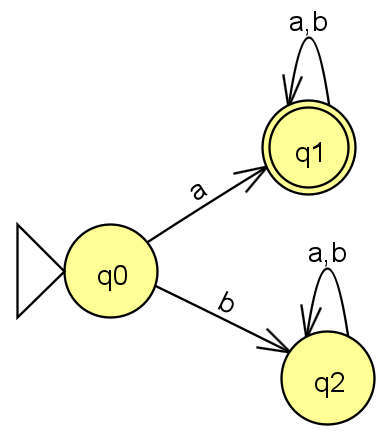
\includegraphics[width=0.2\textwidth]{../../../images/DFAs/ex1_q1.png}



% \vspace{3cm}
% \begin{flushleft}
% أرجو لكم وقتًا ممتعًا.

% الأستاذ محمود اغبارية.
% \end{flushleft}


% \end{document}


\begin{document}

\pagestyle{empty}
\thispagestyle{empty}

%%%%%%%%%%%%%%%%%%%%%%%%%%%%%%%%%%%%%%%%%%%%%%%%
\section*{\underline{موديلات حسابية}}
\begin{enumerate}[label=\arabic*., start=4]

% \subsection*{السؤال الرابع}
\item
نعرّف اللغة $L$ فوق الأبجدية $\{a, b, c\}$ بحيث تحتوي على كلّ الكلمات التي تحقق \underline{على الأقلّ} أحد الشّروط التالية:
\begin{enumerate}[label=(\Roman*)]
    \item تحتوي الكلمة على عدد \underline{فردي} من السلسلة $ac$، \underline{وأيضًا} تنتهي بالسلسلة $acb$.
    \item تحتوي الكلمة على عدد \underline{زوجي} من السلسلة $ac$، \underline{وأيضًا} تنتهي بالسلسلة $cbc$.
\end{enumerate}
\vspace{1em}
\begin{enumerate}
    \item[أ.] لكل واحدة من الكلمات التالية حدد إذا كانت تنتمي للغة $L$ أم لا، إذا كانت تنتمي للغة اكتب أيّ شرط من الشرطين تحقق: \\
    \[ \epsilon \ \ ; \quad acb \ \ ; \quad cbc \ \ ; \quad acbc \ \ ; \quad bacabcacbc \]
    \item[ب.] أثبتوا أنّ اللغة $L$ هي لغة نظامية. عليكم الاستعانة بصفات الانغلاق.
\end{enumerate}

\ifwithsols
\begin{boxSolution}
\begin{itemize}
    \item[أ.]
    \begin{itemize}
        \item $\epsilon$: لا تنتمي.
        \item $acb$: تنتمي، وتحقّق (I).
        \item $cbc$: تنتمي، وتحقّق (II).
        \item $acbc$: لا تنتمي.
        \item $bacabcacbc$: تنتمي، وتحقّق (II).
    \end{itemize}
    \item[ب.]
    نعرّف اللغات الأربع التالية:
    \begin{itemize}
        \item $L_1$: تحتوي على كلّ الكلمات التي تحتوي على عدد زوجي من السلسلة $ac$.
        \item $L_2$: تحتوي على كلّ الكلمات التي تحتوي على عدد فردي من السلسلة $ac$.
        \item $L_3$: تحتوي على كلّ الكلمات التي تنتهي بالسلسلة $acb$.
        \item $L_4$: تحتوي على كلّ الكلمات التي تنتهي بالسلسلة $cbc$.
    \end{itemize}
    نثبت أوّلا أنّ اللغات الأربع هذه هي لغات نظامية:
    \begin{itemize}
        \item اللغة $L_1$ نظامية لأنّ الأوتومات التالي يقبلها:
        \begin{center}
            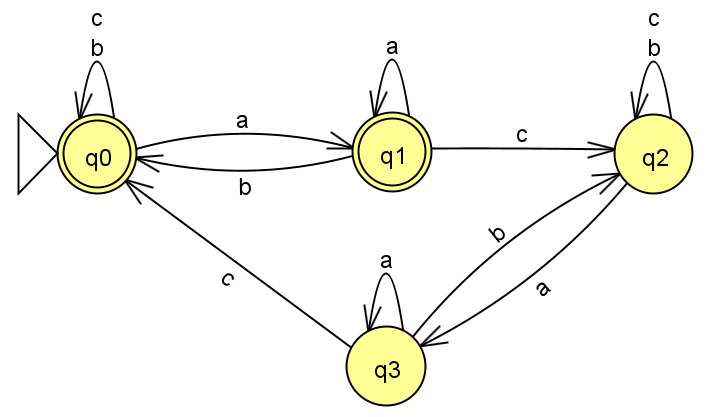
\includegraphics[width=0.5\paperwidth,keepaspectratio]{../../../images/DFAs/even_ac.png}%
        \end{center}
        \item اللغة $L_2$ نظامية لأنّه يتحقق أنّ $L_2 = \overline{L_1}$ وحسب صفات الانغلاق: بما أنّ $L_1$ نظامية، فإنّ $L_2$ نظامية.
\end{itemize}
\end{itemize}
\end{boxSolution}
\clearpage
\begin{boxSolution}
\begin{itemize}[label=-]
    \item اللغة $L_3$ نظامية لأنّ الأوتومات التالي يقبلها:
    \begin{center}
        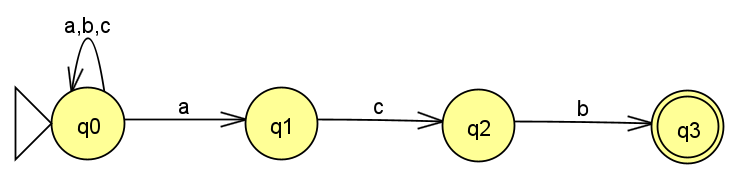
\includegraphics[width=0.5\paperwidth,keepaspectratio]{../../../images/DFAs/ends_with_acb.png}%
    \end{center}
    \item اللغة $L_4$ نظامية لأنّ الأوتومات التالي يقبلها:
    \begin{center}
        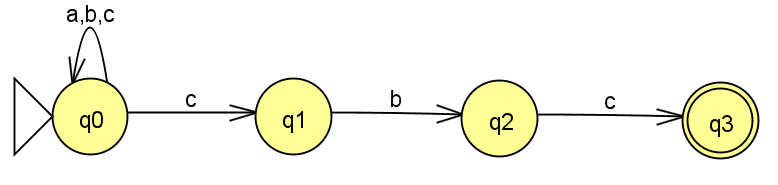
\includegraphics[width=0.5\paperwidth,keepaspectratio]{../../../images/DFAs/ends_with_cbc.png}%
    \end{center}
\end{itemize}
نلاحظ أنّه يتحقق: $L = (L_1 \cap L_4) \cup (L_2 \cap L_3)$. \\
حسب صفات الانغلاق للغات النظامية:
\begin{itemize}
    \item بما أنّ $L_1$ و $L_4$ نظاميتان، فإنّ $L_1 \cap L_4$ نظامية.
    \item بما أنّ $L_2$ و $L_3$ نظاميتان، فإنّ $L_2 \cap L_3$ نظامية.
    \item لذلك $L = (L_1 \cap L_4) \cup (L_2 \cap L_3)$ نظامية لأنّها اتحاد لغتين نظاميتين.
\end{itemize}


\end{boxSolution}
\fi

%%%%%%%%%%%%%%%%%%%%%%%%%%%%%%%%%%%%%%%%%%%%%%%%
\clearpage
% \subsection*{السؤال الخامس}
\item
في هذ السؤال بندان، "أ - ب،" لا علاقة بينهما. أجيبوا عن البندين

\begin{enumerate}
    \item[أ.]
    معطاة ثلاث لغات $L_1$، $L_2$، $L_3$ فوق الأبجديّة $\{a, b\}$. \\
     بالنسبة لكلّ ادّعاء من الادعاءات التالية، اذكروا إذا كان صحيحًا أم غير صحيح. \\
إذا كان الادّعاء صحيحًا - علّلوا لماذا.
وإذا كان غير صحيح - أعطوا مثالًا يُناقضه.
\begin{enumerate}[label=(\arabic*)]
    \item $(L_1 \cap L_2) \bullet L_3 = (L_1 \bullet L3) \cap (L_2 \bullet L_3)$
    \item $R(L_1 \bullet R(L_1)) = L_1 \bullet R(L_1)$
    \item إذا كانت $L_1 \bullet L_2 = L_1 \bullet L_3$، فإنّ $L_2 = L_3$ بالضرورة.
\end{enumerate}

\item[ب.] معطاة اللغة $L$ فوق الأبجدية $\{a, b, c\}$:
$$L = \{ (ab)^n c^{n+m} a^{2m} \mid n,m \ge 1, m\%2=1 \}$$
\begin{enumerate}[label=(\arabic*)]
\item ما هي أقصر كلمة تنتمي للغة $L$؟
\item اكتب كلمتين تنتميان للغة $L$ بحيث يكون طول كل منهما أكثر من 10 أحرف.
\item اكتب كلمتين لا تنتميان للغة $L$ بأي طولٍ كان.
\item ابنوا أوتومات راصة يتلقى اللغة $L$.
\end{enumerate}
\end{enumerate}

\ifwithsols
\begin{boxSolution}

\begin{enumerate}[label=\alph*.]
    \item
\begin{enumerate}[label=(\arabic*)]
    \item صحيح. لأنّ كل كلمة من $(L_1 \cap L_2) \bullet L_3$ هي عبارة عن دمج لكلمة من $L_1 \cap L_2$ مع كلمة من $L_3$. وكذلك كل كلمة من $(L_1 \bullet L3) \cap (L_2 \bullet L_3)$ هي عبارة عن دمج لكلمة من $L_1$ مع كلمة من $L_3$ أو كلمة من $L_2$ مع كلمة من $L_3$.
    \item صحيح. لأنّ $R(X\bullet Y)=R(Y)\bullet R(X)$، وبالتالي
    \[
    R(L_1\bullet R(L_1)) = R(R(L_1)) \bullet R(L_1) = L_1 \bullet R(L_1).
    \]
    \item غير صحيح. مثال: $L_1=\emptyset$، و$L_2=\{a\}$، و$L_3=\{b\}$.
\end{enumerate}
\item
\begin{enumerate}[label=(\arabic*)]
    \item أقصر كلمة: $abccaa$.
    \item مثالان: $abababccccaa$ ، $abccccaaaaaa$.
    \item مثالان: $abcca$ ، $abc$.
    \item .
    \begin{center}
        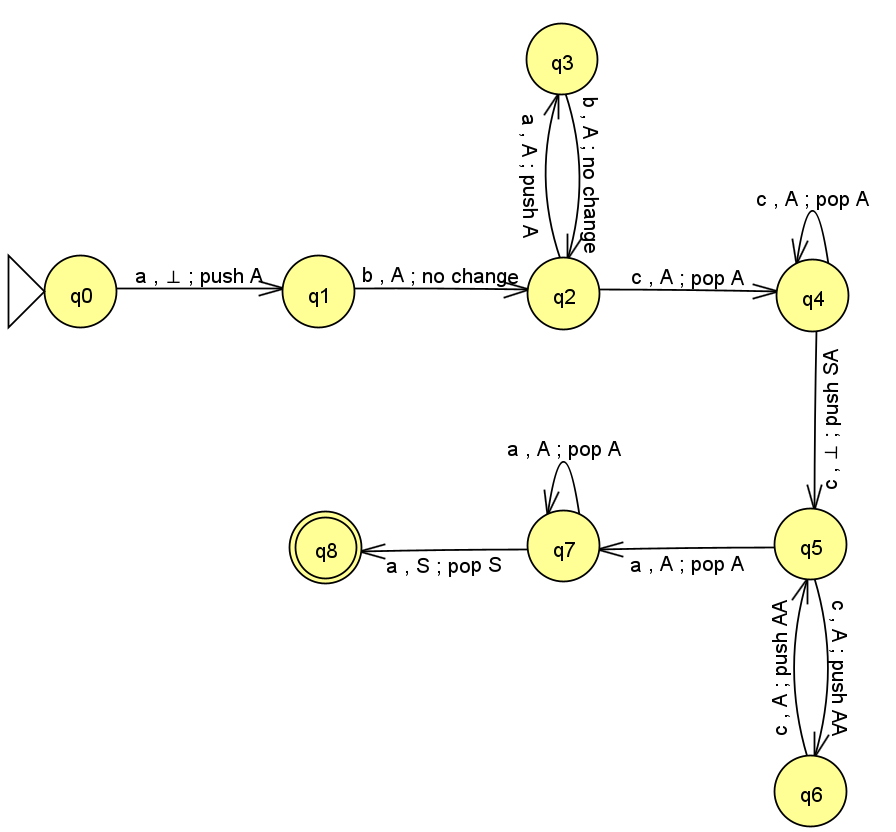
\includegraphics[width=0.7\paperwidth,keepaspectratio]{../../../images/PDAs/abn_cnPm_a2m.png}%
    \end{center}
\end{enumerate}
\end{enumerate}
\end{boxSolution}
\fi
%%%%%%%%%%%%%%%%%%%%%%%%%%%%%%%%%%%%%%%%%%%%%%%
\clearpage
% \subsection*{السؤال السادس}
\item
معطاة العملية الخارجية التالية بلغة C\#:
\begin{boxCode}
\begin{english}
\begin{minted}{csharp}
public static int Foo(int x, int y)
{
    return 2 * x + (y % 2);
}
\end{minted}
\end{english}
\end{boxCode}

تتلقّى آلة تيورينج في بداية الشريط عددين أوناريّين $x$ و $y$ بينهما الرّمز \#،
وتُعيد قيمة العملية $Foo(x, y)$ بين إشارتَي \$ على مكان ما في الشريط.

\begin{enumerate}

\item[أ.] اكتبوا ماذا سيكون الناتج على الشريط في نهاية تشغيل الآلة على المدخل التالي:

\begin{center}
\begin{english}
\begin{tabular}{|c|c|c|c|c|c|c|c|c|}
\hline
$\vdash$ & 1 & 1 & \# & 1 & 1 & 1 & 1 & $\triangle$ \ldots \\
\hline
\end{tabular}
\end{english}
\end{center}

\item[ب.] اكتبوا ماذا سيكون الناتج على الشريط في نهاية تشغيل الآلة على المدخل التالي:

\begin{center}
\begin{english}
\begin{tabular}{|c|c|c|c|c|c|c|c|}
\hline
$\vdash$ & 1 & 1 & \# & 1 & 1 & 1 & $\triangle$ \ldots \\
\hline
\end{tabular}
\end{english}
\end{center}

\item[ج.] اكتبوا آلة تيورينج تُنفّذ العمليّة \textenglish{Foo(x, y)} الموصوفة أعلاه.

توجيهات:
\begin{itemize}
    \item العدد المُعاد يظهر في مكان ما في الشريط بين إشارتَي \$.
    \item لا حاجة لفحص سلامة المُدخَلات.
\end{itemize}

\end{enumerate}
\end{enumerate}

\ifwithsols
\begin{boxSolution}

\begin{enumerate}[label=\alph*.]
    \item .
    \begin{center}
    \begin{english}
    \begin{tabular}{|c|c|c|c|c|c|c|}
    \hline
    $\vdash$ & \$ & 1 & 1 & 1 & 1 & \$ \\
    \hline
    \end{tabular}
    \end{english}
    \end{center}
    \item .
    \begin{center}
    \begin{english}
    \begin{tabular}{|c|c|c|c|c|c|c|c|}
    \hline
    $\vdash$ & \$ & 1 & 1 & 1 & 1 & 1 & \$ \\
    \hline
    \end{tabular}
    \end{english}
    \end{center}
    \item .
    \begin{center}
        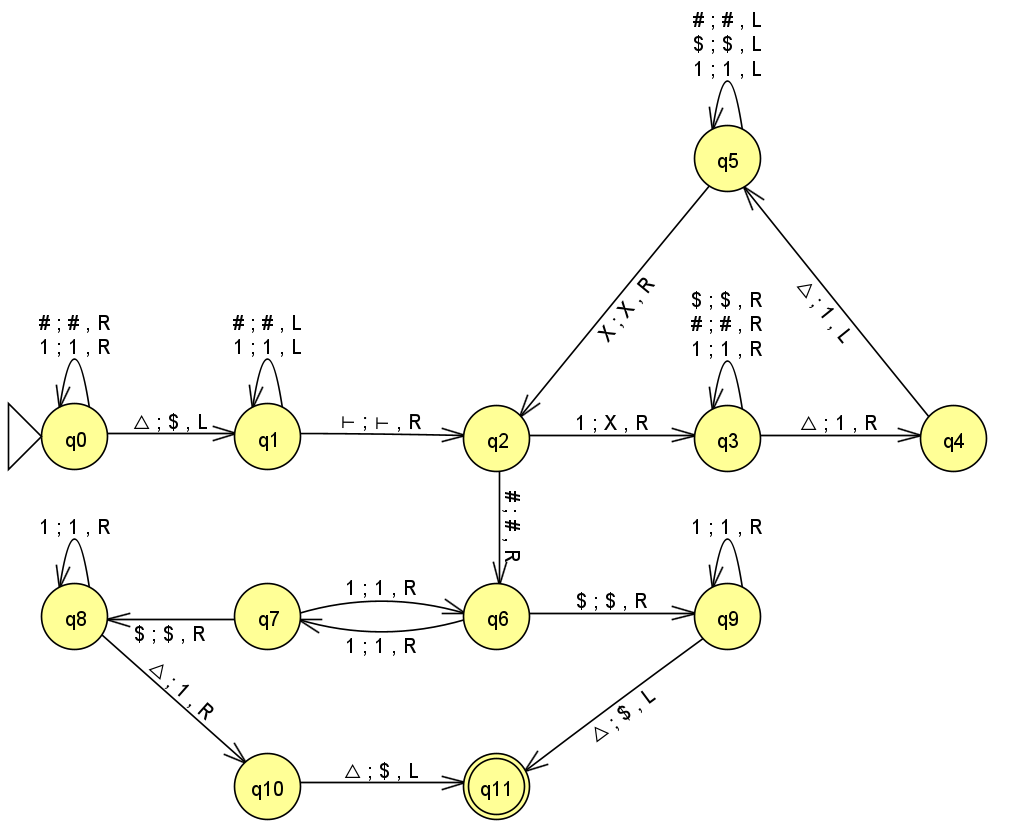
\includegraphics[width=0.7\paperwidth,keepaspectratio]{../../../images/turing/2xPlusYmod2.png}%
    \end{center}
\end{enumerate}

\end{boxSolution}
\fi

\vfill
\begin{center}
نرجو لكم النجاح والتوفيق

معلمو الموضوع
\end{center}

\end{document}